\chapter{Equivalence Checking of Bit-Level Arithmetic Circuits over $\mathbb{F}_{2^k}$} \label{ch:ecbit}

%Computer algebra techniques have been utilized \cite{lv:date2012} \cite{wienand:cav08} to 
%efficiently solve equivalence verification of arithmetic circuits over Ring ${\mathbb{Z}}_{2^k}$ and 
%Finite field ${\mathbb{F}}_{2^k}$ respectively. These computer algebra based approaches have 
%shown their superority over contemporary BDD/SAT/SMT based methods. 
%The efficiency of \cite{lv:date2012} \cite{wienand:cav08} is achieved by converting 
%an equivalence checking problem to ideal membership testing problem. Combined with 
%circuit topology, the ideal membership testing is further transformed to one single 
%polynomial reduction (polynomial division). Therefore, the stunning results of 
%\cite{lv:date2012} \cite{wienand:cav08} introduce a novel way to solve equivalence 
%verification problem with significant orders of magnitude improvement in runtime. 
%However, \cite{lv:date2012} \cite{wienand:cav08} requires a word level specification 
%to verify against bit-level implementation. This word level information is not always 
%available. In other words, not all specifications can be expressed at word level. 

%To overcome this limitation, we draw inspirations from \cite{lv:date2012} \cite{wienand:cav08}, 
%and derive a general verification approach effective at bit level.


The combinational circuit equivalence checking problem has been widely investigated. 
In particular, for synthesized circuits, this problem can
be efficiently solved using the techniques of And-Invert-Graph (AIG) 
based reductions \cite{abc} and circuit-SAT solvers \cite{csat}. 
However, when the circuits are functionally equivalent 
but structurally very dissimilar, none of the contemporary techniques, 
including BDD/SAT/SMT/ABC, are able to prove equivalence. 
Since these custom designed circuits are prevalent in industry, 
it is therefore imperative to develop scalable verification methods to verify such circuits. 

By utilizing computer algebra theory, we formulate this problem as a weak Nullstellensatz proof using Gr\"obner bases computation. 
Once again, this would require the computation of a reduced Gr\"obner basis, which is expensive for large circuits. 
To overcome this complexity, we want to exploit our circuit-based term ordering for polynomial representation. 
Unfortunately, unlike in the previous case in last chapter, the set of polynomials corresponding to this verification instance does 
not constitute a Gr\"obner basis. Instead of computing a Gr\"obner basis for the the whole circuit, 
we identify a minimal number of S-polynomial computations that are sufficient to prove equivalence or 
to detect bugs for the whole circuit.
Experiments show the effectiveness and efficiency of our approach: 
we can verify $96$-bit structurally very dissimilar implementations.

%%%%%%%%%%%%%%%%%%%%%%%%%%%%%%%%%%%%%%%%%%%%%%%%%%
%%%%%%%%%%%%%%%%%%%%%%%%%%%%%%%%%%%%%%%%%%%%%%%%%%
%%%%%%%%%%%%%%%%%%%%%%%%%%%%%%%%%%%%%%%%%%%%%%%%%%
\section{Problem Statement and Modeling}

In this application, we are given two combinational arithmetic circuits $C_{1}$ and $C_{2}$, as gate-level flattened netlists.
We have to prove or disprove their functional equivalence. 

Our approach is generic enough to conduct equivalence checking of combinational arithmetic circuits over $\mathbb{F}_{2^k}$.
Again, without loss of generality, we utilize multiplier circuits as examples to explain our approach.

Our problem can be formally described as:

\begin{itemize}
\item Given a finite field $\mathbb{F}_{2^k}$, i.e. given $k$ (datapath size), along with the
  corresponding irreducible polynomial $P(x)$. Let $P(\alpha) = 0$, i.e. $\alpha$ be the root of $P(x)$.  
\item  Given two $k$-bit combinational circuits $C_{1}$ and $C_{2}$. 
		The common primary inputs of both circuits are $\{a_0, \dots, a_{k-1}, ~b_0,\dots, b_{k-1}\}$. 
		The primary outputs of $C_{1}$ are $\{x_0, \dots, x_{k-1}\}$;
		The primary outputs of $C_{2}$ are $\{y_0, \dots, y_{k-1}\}$, 
		where $a_i, b_i, x_i, y_i\in \mathbb{F}_2, i = 0, \dots, k-1$.
		Correspondingly, the word-level representation of outputs are
		$X = x_0 + x_1\alpha  + \dots +  x_{k-1}\alpha^{k-1}$ adn $Y = y_0 + y_1\alpha  + \dots +  y_{k-1}\alpha^{k-1}$, respectively.
\end{itemize}
Our goal is to formally prove that $\forall a_{i},b_{i} \in \mathbb{F}_{2} \subset \mathbb{F}_{2^k}$,
the outputs $X$ and $Y$ of circuits $C_{1}$ and $C_{2}$ are equal to each other, 
i.e., $ X=Y$ always holds. Otherwise, there must exist a bug in one of the given circuits.  


\begin{figure}[htb]
\centerline{
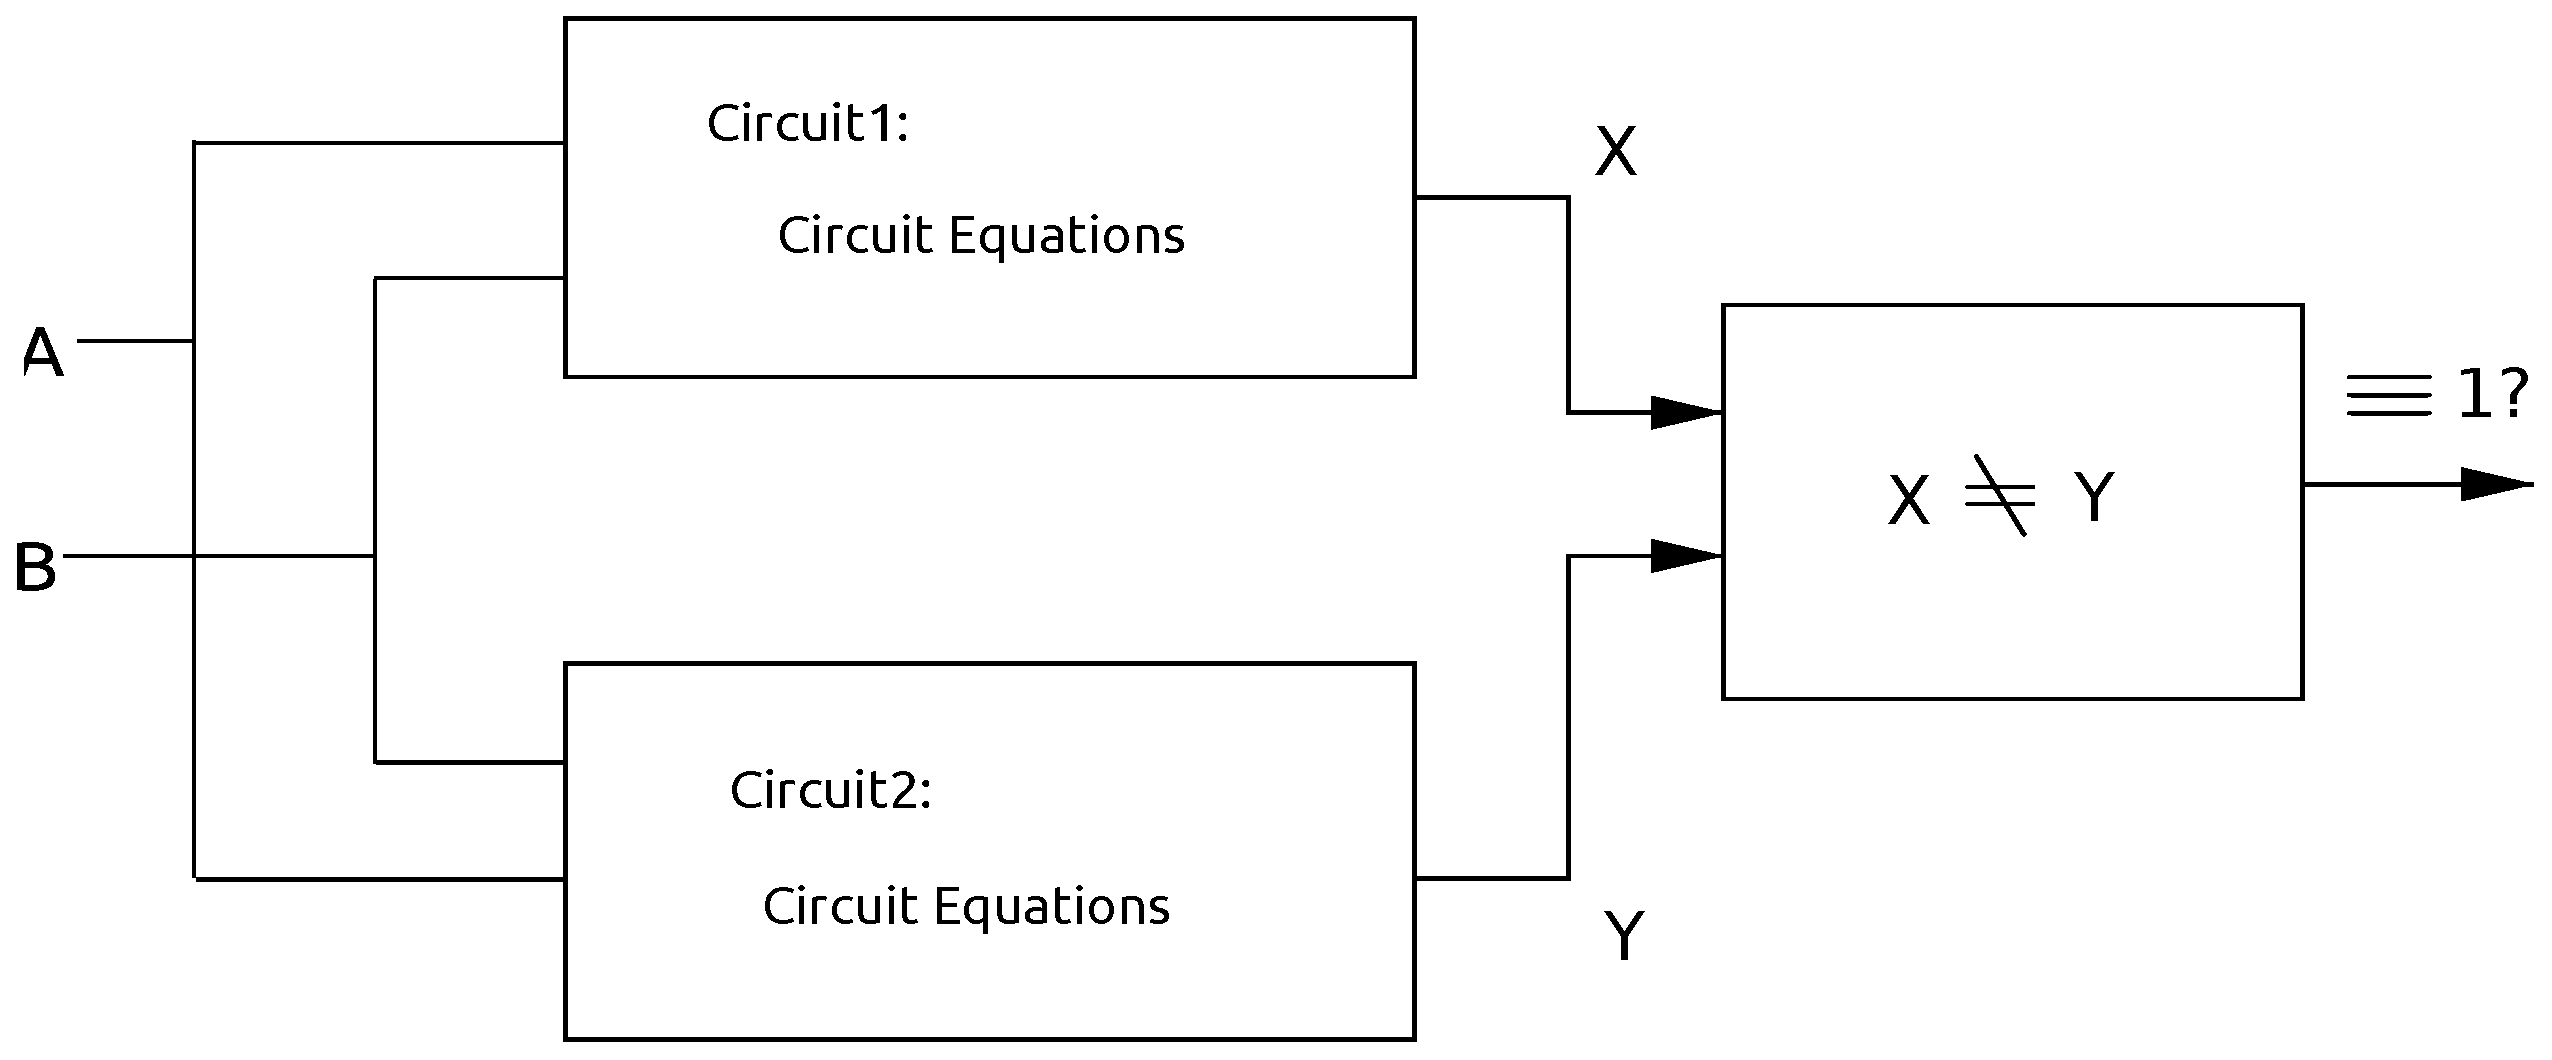
\includegraphics[scale=0.3]{./figures/miter.eps}
}
\caption{The Equivalence Checking Setup: Miter}
\label{fig:miter}
\end{figure}

The equivalence verification setup is shown in Fig. \ref{fig:miter}. 
Given circuits $C_{1}$ and $C_{2}$, 
we want to prove that for all possible inputs, 
the output $X$ of circuit $C_{1}$ is always equal to the output $Y$ of circuit $C_{2}$ . 
This can be, conversely, modeled as as a miter, i.e., $X \neq Y$ has no solutions. 
Such a setup is a standard practice in combinational circuit verification, 
because this enables the use of {\it constraint-solvers} (such as SAT, SMT, etc.) to prove/disprove equivalence. 
The $X\neq Y$ constraint is further modeled as a polynomial over
$\mathbb{F}_{2^k}$ as follows:
\begin{equation}
t(X - Y) = 1, \text{where $t$ is a free variable in }\mathbb{F}_{2^k}.  
\end{equation}
 The correctness of the above
constraint modeling can be shown as follows: 
\begin{itemize}
	\item When $X = Y, X-Y =0$, so $t\cdot 0 = 1$ has no solutions.
	\item When $X\neq Y, (X-Y) \neq 0$. Over any field, every non-zero element has a multiplicative
		inverse. Let $t^{-1} = (X-Y)$. Then $t \cdot t^{-1} = 1$ will always have a solution over $\mathbb{F}_{2^k}$.
	\item As a special case over $\mathbb{F}_2$, since $1$ is the only non-zero element $X\neq G$ is formulated as $X+Y+1 \pmod 2$.	
\end{itemize} 
If indeed there are no solutions to $X \neq Y$, then it
implies that $X$ is always equal to $Y$. Otherwise, 
if there is a solution to our problem instance, then there is an assignment where
$X$ differs from $Y$ which indicates a bug in the circuit.   

Following the mapping rules given in Equations \ref{b2poly}, 
the circuit equations are transformed into polynomial representation.

Overall, the miter circuit can be modeled as a polynomial system over $\mathbb{F}_{2^k}$:

\begin{eqnarray}\label{eqn:miterbit}
 \left .  \begin{aligned}
f_1^{1}(x_1,x_2,\cdots, x_d)  \\
\vdots  \\
f_{X}: X+x_{0}+x_{1}\cdot \alpha+\dots+ x_{k-1}\cdot \alpha^{k-1} \\
%f_{Z}: Z+z_{0}+z_{1}\cdot \alpha,\cdots,{z_{k-1}}\cdot \alpha^{k-1}=0   
 \end{aligned} 
\ \right\}
 &\qquad&  \text{\it Circuit $1$} \nonumber \\
 \left . \begin{aligned}
f_1^{2}(x_1,x_2,\cdots, x_d)=0  \\
\vdots  \\
f_{Y}: Y+y_{0}+y_{1}\cdot \alpha+\dots+ y_{k-1}\cdot \alpha^{k-1} \\
 \end{aligned} 
\right\}
 &\qquad&  \text{\it  Circuit $2$}  \\
 \left .  \begin{aligned}
f_{m}:t\cdot (X-Y)+1=0  \nonumber 
 \end{aligned} 
\right\}
 &\qquad& \text{Miter:}X \neq Y \nonumber 
\end{eqnarray}

We use the following example to illustrate our polynomial system modeling.

\begin{Example}\label{exp:miter}
	Consider two functionally equivalent circuits implementing $2$-bit adder over $\mathbb{F}_{2}$.
	The miter circuit is given in Figure \ref{fig:2bitadder}.
	\begin{figure}[htb]
		\centerline{
		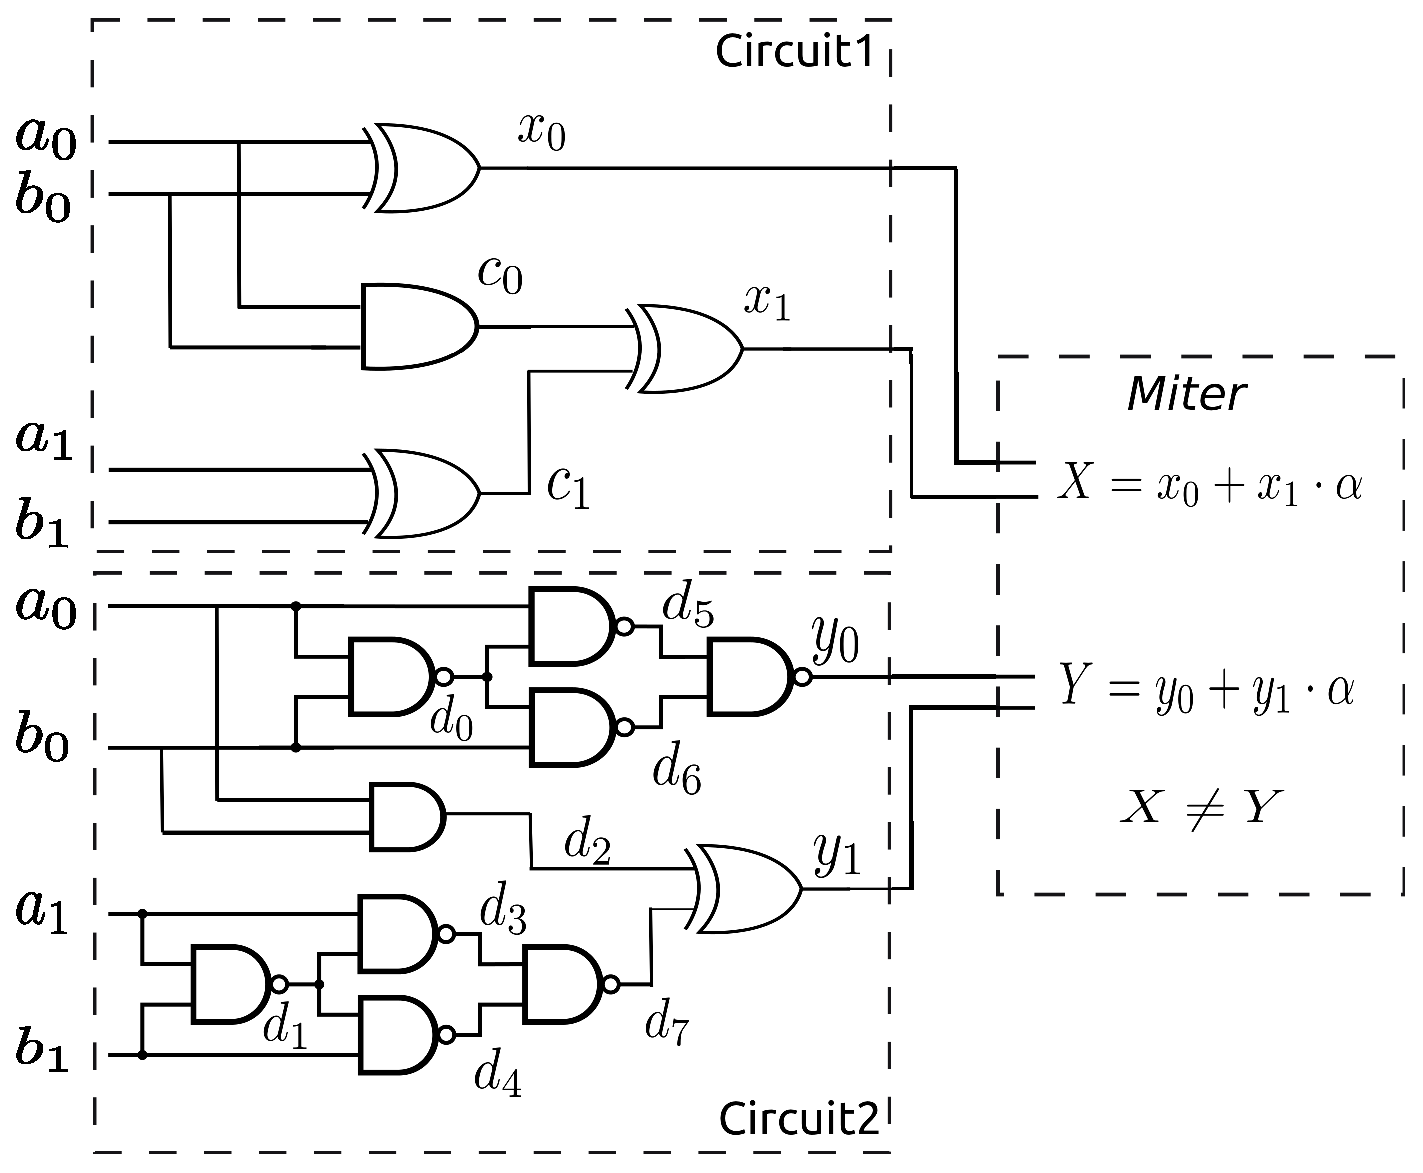
\includegraphics[scale=0.5]{./figures/2bitadder.eps}
		}
		\caption{Miter for $2$-bit Adders.}
		\label{fig:2bitadder}
	\end{figure}

	Then the miter circuit described in Figure \ref{fig:2bitadder} is modeled as a system of polynomials.
	Note that the outputs is expressed at word level as: $X+x_{0}+x_{1}\cdot \alpha$ and $Y+y_{0}+y_{1}\cdot \alpha	$.

\begin{eqnarray}[htb]
 \left .  \begin{aligned}
	x_0&=a_0 \oplus b_0  \Rightarrow x_0+a_0 + b_0 \\
	c_0&=a_0\wedge b_0   \Rightarrow c_0+a_0 \cdot b_0\\
	c_1&=a_0\oplus b_1   \Rightarrow c_1+a_0 + b_1 \\
	x_{1}&=c_{0}\oplus c_{1}  \Rightarrow x_{1}+c_{0}+ c_{1} \\
	&X+x_{0}+x_{1}\cdot \alpha				\\
	 \end{aligned} 
\ \right\}
 &\qquad&  \text{\it Circuit $1$} \nonumber \\
 \left . \begin{aligned}
d_{0}&=\neg (a_{0} \wedge b_{0}) \Rightarrow d_{0}+ a_{0} \cdot b_{0}+1  \\
	d_{1}&=\neg (a_{1} \wedge b_{1}) \Rightarrow d_{1}+ a_{1} \cdot b_{1}+1  \\
	d_{2}&= a_{0} \wedge b_{0} \Rightarrow d_{2}+ a_{0}\cdot b_{0} \\
	d_{3}&=\neg (a_{1} \wedge d_{1}) \Rightarrow d_{3}+ a_{1} \cdot d_{1}+1  \\
	d_{4}&=\neg (b_{1} \wedge d_{1}) \Rightarrow d_{4}+ b_{1} \cdot d_{1}+1  \\
	d_{5}&=\neg (a_{0} \wedge d_{0}) \Rightarrow d_{5}+ a_{0} \cdot d_{0}+1  \\
	d_{6}&=\neg (b_{0} \wedge d_{0}) \Rightarrow d_{6}+ b_{0} \cdot d_{0}+1  \\
	d_{7}&=\neg (d_{3} \wedge d_{4}) \Rightarrow d_{7}+ d_{3} \cdot d_{4}+1  \\ 
	y_{0}&=\neg (d_{5} \wedge d_{6}) \Rightarrow y_{0}+ d_{5} \cdot d_{6}+1  \\
	y_{1}&=d_{2} \oplus d_{7}   \Rightarrow  y_{1}+d_{2} + d_{7}	\\
	&Y+y_{0}+y_{1}\cdot \alpha				\\
 \end{aligned} 
\right\}
 &\qquad&  \text{\it  Circuit $2$} \nonumber \\
 \left .  \begin{aligned}
	&t\cdot (X-Y)+1=0 				
 \end{aligned} 
\right\}
 &\qquad& \text{Miter:}X \neq Y
\end{eqnarray}

\end{Example}


With the polynomial model given above, we formulate our problem as a {\bf Weak Nullstellensatz} problem, 
which is described next.

%%%%%%%%%%%%%%%%%%%%%%%%%%%%%%%%%%%%%%%%%%%%%%%%%%%%%%%%%%%%%%%%
%%%%%%%%%%%%%%%%%%%%%%%%%%%%%%%%%%%%%%%%%%%%%%%%%%%%%%%%%%%%%%%%
%%%%%%%%%%%%%%%%%%%%%%%%%%%%%%%%%%%%%%%%%%%%%%%%%%%%%%%%%%%%%%%%
\subsection{Verification Problem Formulation as Weak Nullstellensatz}

As described in Equation \ref{eqn:miterbit} and Example \ref{exp:miter},
to formulate our verification test, we first analyze the miter circuit and 
model the Boolean gate-level operators as polynomials over $\mathbb{F}_2$
-- i.e. two set of implementation polynomials representing $C_{1}$ and $C_{2}$, 
and the miter polynomials: $X \neq Y$ ($X,Y$ are outputs of $C_{1}$ and $C_{2}$). 
Subsequently, we can reason whether or not solutions exist
to this polynomial system. 

For this purpose, we wish to use techniques from computer algebra and algebraic Geometry to reason about the
solutions (variety) to the polynomial equations (ideal). 

Let $F_1, F_2$ represent polynomials generated from circuit $C_1$ and $C2$ respectively.
Let $f_m$ represent the miter polynomial.
Let $F=\{F_1,F_2,f_m\}=\{f_1,f_2,\ldots,f_s\}$ denote this set of polynomials derived from the miter circuit. 
Let $\{x_1,\dots,x_d\}$ denote all variables occurring in $F$.
Let $J = \langle F_1,F_2,f_s\rangle \subset \mathbb{F}_{2^k}[x_{1},\dots,x_{d}]$ denote the ideal generated by these polynomials.
Subsequently, $V(J)$ denotes the variety (solutions) of $J$ over .
Our verification problem can be formulated as the evaluation:
\begin{equation}
V(\langle J\rangle)=\emptyset?
\end{equation}
A direct answer is {\bf Weak Nullstellensatz} \cite{null:1890}.


{\it Weak  Nullstellensatz} explicitly specifies the condition when variety is empty.

%%%%%%%%%%%%%%%%weak nullstellensatz%%%%%%%%%%%%%
\begin{Theorem}
$\left[\bf{Weak\  Nullstellensatz}\right]$ Let $J \subset \overline {\mathbb{K}}[x_1, x_2, \cdots, x_d]$ be an ideal satisfying $V(J)=\emptyset$. 
Then $I=\overline {\mathbb{K}}[x_1, x_2, \cdots, x_n] \iff \{1\} \in J$.
\end{Theorem}

Recall that a reduced Gr\"obner basis is a canonical representation of an ideal. 
From the definition of ideal, we know that ideal $\langle 1 \rangle$ can 
generate all polynomials in $\mathbb{K}[x_1, x_2, \cdots, x_n]$. 
Therefore, Weak Nullstellensatz can be further described as:
\begin{Corollary}\label{cor:wnf2}
$\left[\bf{Weak\  Nullstellensatz}\right]$ Let $I \subset \overline {\mathbb{K}}[x_1, x_2, \cdots, x_d]$ be an ideal satisfying $V(I)=\emptyset$. 
Then Reduced Gr\"obnerBasis(I)$=\{1\}$.
\end{Corollary}

The {\it Weak Nullstellensatz} now offers us a way to evaluate whether the system of multivariate polynomial equations has a common solution 
in ${\overline {\mathbb{K}}}^d$.

However, {\it Weak Nullstellensatz} is stated over an algebraically closed field.
Our problem is modeled over $\mathbb{F}_{2^{k}}$ which is not an algebraically closed field. 
So {\it Weak Nullstellensatz} will bound to fail when applying to finite field.

Let us explain why {\it Weak Nullstellensatz} fails when applying to the field $F_{2}\subset F_{2^{k}}$ by an example.
\begin{Example} \label{exp:wnfail}
We are given an implementation of a circuit over $\mathbb{F}_2 \subset \mathbb{F}_{2^{k}}$: 
\begin{equation}
x_1=a \vee (\neg a \wedge b)
\end{equation}
Its corresponding specification is :
\begin{equation}
y_1=a \vee b
\end{equation}
$x_1$ and $y_1$ are symbolically different but functionally equivalent.  
Then we transform the circuit equations into their polynomial forms:
\begin{eqnarray}
x_1=a \vee (\neg a \wedge b) &\mapsto& x_1 + a + b\cdot (a+1) + a\cdot b \cdot (a+1) \pmod 2 \nonumber \\
y_1=a \vee b  &\mapsto& y_{1}+a+b+a\cdot b \pmod 2 \nonumber \\
x_1 \neq y_{1}  &\mapsto& x_1+y_1+1 \pmod 2 \nonumber
\end{eqnarray}
\end{Example}
Then Gr\"obner basis of above polynomials with term ordering {\it lp}:$x_{1}>y_{1}>a>b$ is: 
\begin{eqnarray}
a^{2}\cdot b+a \cdot b+1 \nonumber \\
y_{1}+a \cdot b+a+b \nonumber \\
x_{1}+a \cdot b+a+b+1 \nonumber 
\end{eqnarray}

which is supposed to be $\langle 1\rangle$. The reason is explained as follows.
As shown in Figure \ref{fig:closure}. 
\begin{figure}[htb]
\centerline{
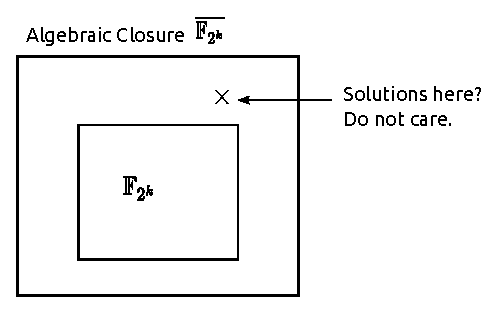
\includegraphics[scale=1]{./figures/closure.eps}
}
\caption{ A Solution (Bug) in $(\overline{\mathbb{F}_{2^{k}}}-\mathbb{F}_{2^k})$ is a ``don't care''.}
\label{fig:closure}
\end{figure}

If there is no solution in the algebraic closure $\overline{ \mathbb{F}_{2^k}}$, 
then there is no solution in $\mathbb{F}_{2^k}$ either. However, what
happens when there is a solution in $\overline{ \mathbb{F}_{2^k}}$, namely $1 \notin GB(J)$? 
In this case, it means that there is a
{\it non-empty set of  solutions (finite or infinite)} to the
polynomial system in $\overline{\mathbb{F}_{2^k}}^d$. There are two possibilities: 
\begin{itemize}
	\item The solution(s) may lie within $\mathbb{F}_{2^k}^d$.
	\item The solution(s) may lie in $\overline {\mathbb{F}_{2^k}}^d$, but outside $\mathbb{F}_{2^k}^d$, as depicted in  Fig. \ref{fig:closure}.
\end{itemize}
We are interested in finding out whether or not $X \neq Y$ over $\mathbb{F}_{2^{k}}$ 
-- i.e. whether the circuit has bugs over the given field $\mathbb{F}_{2^{k}}$. We do not care if the
solution is outside the field $\mathbb{F}_{2^{k}}$, in which case the bug is really a
``don't care'' condition (akin to a ``false negative'' in design verification parlance). 



To solve this problem, {\it Weak Nullstellensatz} needs to be suitably modified for application over finite fields $\mathbb{F}_{2^{k}}$.
%%%%%%%%%%%%%%%%weak nullstellensatz in finite field%%%%%%%%%%%%%
\begin{Theorem}\label{wnull:ff}
$[\bf{Weak~Nullstellensatz~in~\mathbb{F}_{2^k}}]$\\
Given $f_1,f_2,\cdots,f_s \in \mathbb{F}_{2^k}[x_1,x_2,\cdots,x_d]$. 
Let $J=\langle f_1,f_2,\cdots,f_s\rangle \subset \mathbb{F}_{2^k}[x_1, x_2, \cdots, x_d]$ be an ideal. 
If $V_{\mathbb{F}_{2^k}}(J)=V_{\overline {\mathbb{F}_{2^k}}}(J,x_1^{2^k}-x_1,x_2^{2^k}-x_2,\cdots,x_d^{2^k}-x_d)=\emptyset$, 
then reduced Gr\"obnerBais$(J+J_{0})=\{1\}$.
\end{Theorem}
 
\begin{Proof}
For convenience, let $J_0$ denote $x_1^{2^k}-x_1,x_2^{2^k}-x_2,\cdots,x_d^{2^k}-x_d$.

According to definition of vanishing polynomials over $\mathbb{F}_{2^k}$, we have
$V_{\overline {\mathbb{F}_{2^k}}}(J_0)={\mathbb{F}_{2^k}^d}$, 

From Lemma \ref{lem:closure}, we know:
\begin{equation}
	V_{\overline {\mathbb{F}_{2^k}}}(J+J_0)=V_{\mathbb{F}_{2^k}}(J). 
\end{equation}

Combining with Corollary \ref{cor:wnf2}: 
\begin{equation}
V_{\overline {\mathbb{F}_{2^k}}}(J+J_0)=\emptyset \Leftrightarrow \text{Gr\"obnerBais(J+$J_0$)} =\langle 1\rangle 
\end{equation}
we can finalize our conclusion:
\begin{equation}
V_{\overline {\mathbb{F}_{2^k}}}(J+J_0)=V_{\mathbb{F}_{2^k}}(J)=\emptyset \Leftrightarrow {\text{Reduced Gr\"obnerBais(J+$J_{0}$)}}=\{ 1\}  \nonumber
\end{equation}
{}
\end{Proof}

\begin{Example}
Let us re-visit Example \ref{exp:wnfail}, we append vanishing polynomials $a^2-a,b^2-b,x_1^2-x_1,y_1^2-y_1$ to original ideal. 
Then we get: $GB(x_1+ a + b\cdot(a+1) + a\cdot b\cdot(a+1),y_1+a+b+a\cdot b,x_1+y_1+1,a^2-a,b^2-b,x_1^2-x_1,y_1^2-y_1)=\{1\}$ which indicates $x_1=y_1$.
\end{Example}


{\bf Verification Problem Formulation:}
Through Weak Nullstellensatz over $\mathbb{F}_{{2^k}}$, given an ideal $J \in \mathbb{F}_{2^k}[x_{1},\dots,x_{d}]$, 
we can determine whether the variety of $J$ is empty by analyzing the corresponding reduced Gr\"obner basis.

For our verification problem, we take the polynomials $\{f_1, \dots, f_s\}$ 
representing the miter circuit constraints to generate ideal $J$.
Then we append the vanishing polynomials $\{x_1^{2^k} - x_1, \dots, x_d^{2^k} - x_d\}$ of ideal $J_0$.
Therefore, to check if a system of polynomial equations
has no solutions, we need to compute the reduced Gr\"{o}bner basis $G$ of $J+J_0$
and check if $G$ equals to the unit ideal $\langle 1 \rangle$.
If $G=\{1\}$, two circuits are functionally equivalent. Otherwise, there must a bug in the design.

Similar to ideal membership testing, the critical step of Weak Nullstellensatz formulation is to compute a Gr\"obner basis.
However, the complexity of Gr\"obner basis makes such a computation infeasible. 
To overcome this complexity, we again want to exploit our circuit-based term ordering for polynomial representation. 
Unfortunately, under Weak Nullstellensatz formulation, the set of polynomials corresponding to this verification instance does not constitute 
a Gr\"obner basis, as shown by Example \ref{exp:1bitmiter}. 

%\begin{Example}\label{exp:1bitmiter}
	
%\begin{figure}[hbt]
%\centerline{
%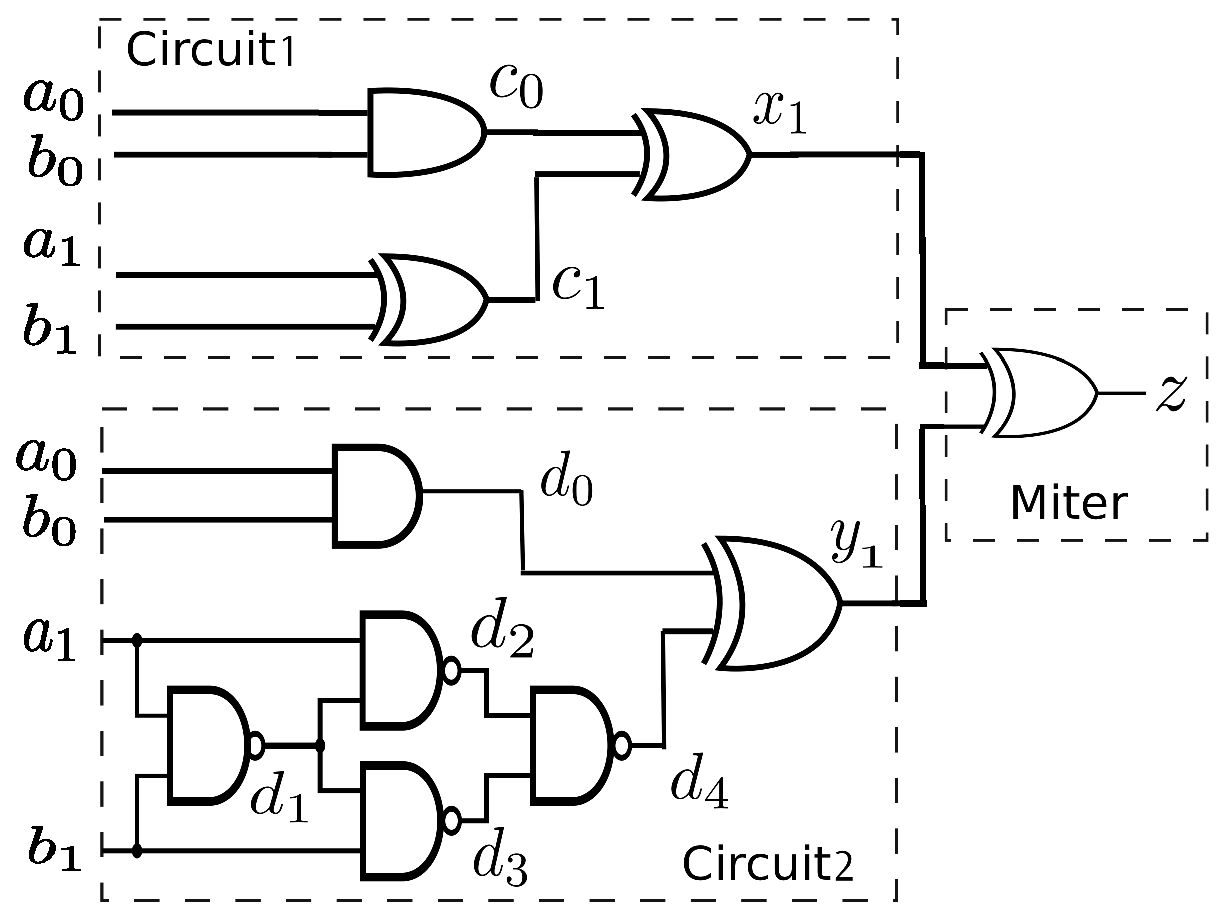
\includegraphics[scale=0.40]{./figures/1bitmiter.eps}
%}
%\caption{Miter}
%\label{fig:1bitmiter}
%\end{figure}

%The above two circuits are functiaonally equivalent and their polynomials are described as follows:


%\begin{eqnarray}
 %\left .  \begin{aligned}
	%& c_0 + a_0\cdot b_0   \\
	%& c_1 + a_1 + b_1   \\
	%& x_1 + c_0 + c_1   \\
	 %\end{aligned} 
%\ \right\}
 %&\qquad&  \text{\it Circuit $1$: $F_{1}$} \nonumber \\
 %\left . \begin{aligned}
	%&d_0+a_0 \cdot b_0 \\
	%&d_1+a_1\cdot b_1+1   \\
	%&d_2+ a_1\cdot d_1+1   \\
	%&d_3+ b_1\cdot d_1+1  \\
	%&d_4+d_2\cdot d_3			\\
	%&y_1+d_0+ d_4   		\\
 %\end{aligned} 
%\right\}
 %&\qquad&  \text{\it  Circuit $2$}: F_{2}  \\
 %\left .  \begin{aligned}
	%& x_1 + y_1 + 1  			
 %\end{aligned} 
%\right\}
 %&\qquad& \text{Miter $f_{m}$:}X \neq Y \nonumber
%\end{eqnarray}
\begin{Example}\label{exp:1bitmiter}
Let us re-consider Example \ref{exp:wnfail}. Based on the {\it optimal term ordering} of the circuit: \\
$ x_1 >  y_1 > d_4 > d_3 > d_2 > d_1> d_0 >c_1 > c_0 > a_0 > a_1 > b_0 > b_1$, \\ 
Ideal $\langle F_{1},F_{2}, f_{s} \rangle$ does not constitutes a Gr\"obner Basis.
Because miter polynomial $t\cdot X-t\cdot Y+1$ and output polynomial of circuit $C_1$ $X+x_0+x_1\cdot \alpha$ has a common leading variable $X$
between their leading terms $t\cdot X$ and $X$,
thus violating the property of Gr\"obner Basis: all leading terms should be relatively prime.  
\end{Example}


In the next section, we describe an approach that can identify a minimal number of S-polynomial computations that
are sufficient and necessary to prove equivalence or to detect bugs.

%%%%%%%%%%%%%%%%%%%%%%%%%%%%%%%%%%%%%%%%%%%%%%%%%%%%%%%%%%%%%%%%%%%%
%%%%%%%%%%%%%%%%%%%%%%%%%%%%%%%%%%%%%%%%%%%%%%%%%%%%%%%%%%%%%%%%%%%%
%%%%%%%%%%%%%%%%%%%%%%%%%%%%%%%%%%%%%%%%%%%%%%%%%%%%%%%%%%%%%%%%%%%%
\section{Verification Using a Minimal Number of S-polynomial Computation}


Let $F_1, F_2$ represent polynomials generated from circuit $C_1$ and $C2$ respectively.
Let $f_m$ represent the miter polynomial.
Let $F=\{F_1,F_2,f_m\}=\{f_1,f_2,\ldots,f_s\}$ denote this set of polynomials derived from the miter circuit. 
Let $\{x_1,\dots,x_d\}$ denote all variables occurring in $F$.
Let $J = \langle F_1,F_2,f_s\rangle \subset \mathbb{F}_{2^k}[x_{1},\dots,x_{d}]$ denote the ideal generated by these polynomials.
Let $f_o \in F$ denote the polynomial satisfying that $lm(f_0)$ and $lm(f_m)$ are not relatively prime. 
Such a polynomial always exis because the leading term of miter polynomial $f_{m}$ always corresponds 
to the output of either circuit $C_1$ or $C2$. 
Let $T=\{x_1,\dots,x_d\}$ denote all variables occurring in $F$, of which, let $T_{PI}$ denote the primary inputs.

To derive the minimal number of S-polynomial computations for our problem, 
we first consider a pair of polynomials that are not relatively prime: $f_{m}$ and $f_{o}$.
In Example \ref{exp:wnfail}, $f_o=X+x_0+x_1\cdot \alpha$ and $f_m=t\cdot X-t\cdot Y+1$. 
Because of the existence of $f_{m}$ and $f_{o}$, $\{F_1,F_2,f_m\}$ does not constitute a Gr\"obner basis. 
Note that according to Proposition \ref{prop:top-order}, the polynomials in $\{F_1,F_2\}$ indeed constitutes a Gr\"obner basis.
Therefore, to claim that $f_{m}$ and $f_{o}$ is the only pair of polynomials that needs to be reduced in Gr\"obner basis computation
of $\{ F \}$, we have the following lemma and theorem: 

\begin{Lemma}\label{lem:root}
Let $r \in \mathbb{F}_2[x_1, \dots, x_d]$ be a nonconstant polynomial 
such that every monomial term of $r$ has only variables of degree $1$. 
Then $r$ has a root in $\mathbb{F}_2^d$.
\end{Lemma}

\begin{Proof}
Let $l(r)$ denote the number of nonzero monomials appearing in $r$.

We will perform induction on $l(r)$.

The case $l(r)=1$ is clear.

General case:

Since $l(r) \geq 2$ we can write $r =  r' +M$ where $M$ is a product of monomials. 
After renumbering the variables we can assume that $x_1$ divides $M$.

If $x_1$ divides $r'$ then $x_1$ divides $r$ as well and we have a solution for $r$ (anything with $x_1=0$ works).

If $x_1$ does not divide $r$, then let $r"=\mathcal{F}(0, x_2,\ldots, x_d)$. Since $l(r") < l(r)$ ($M$ disappears), 
by induction there is a solution $(x_2, \dots, x_d)$ for $r"$ which gives a solution $(0, x_2, \ldots, x_d)$ for $r$.
\end{Proof}


\begin{Theorem}\label{thm:miter}
Let $J=\langle F \rangle \subset \mathbb{F}_{2^k}[x_{1},\dots,x_{d}]$ 
on which we impose our circuit-based monomial order $>$.
Then $V_{\mathbb{F}_{2^k}}(J)=\emptyset \iff r=1$, where $r$ is computed as 
$Spoly(f_m,f_o)$ $\stackrel{J,J_0}{\longrightarrow} r$ and $f_m, f_o$ are not relatively prime. 
\end{Theorem}

\begin{Proof}
For convenience, let $q=2^k$; let $GB(J)$ represent the Gr\"obner basis of ideal $J$; let $redGB(J)$ represent the reduced Gr\"obner basis of ideal $J$.
Let $T$ represent all variables occurring in $F$; let $T_{pi}$ denote all primary inputs.

To prove the correctness of this theorem, we need to consider the following two steps:
\begin{enumerate}
\item $GB(J+J_{0})=\{J,J_{0},r\}$, where $r$ is computed as $Spoly(f_m,f_o)$ $\stackrel{J,J_0}{\longrightarrow} r$ and $f_m, f_o$ are not relatively prime. 
		In other words, $r$ is the only generated polynomial in the Gr\"obner Basis computation of $J+J_{0}$.
\item In terms of Theorem \ref{wnull:ff}: $V_{\mathbb{F}_{q}}(J)=\emptyset \iff redGB(J+J_{0})=\{1\}$, we only need to check 
		$redGB(J+J_{0})=\{1\}$ holds.
\end{enumerate}

Let us consider Step $1$.
Since we already know $Spoly(f_m,f_o)$ is the only polynomial that needs to be reduced in the given polynomial set $F$, 
we only need consider whether $r$ will result in another polynomial generated. If $r=1$ or $r=0$, obviously $r$ is relatively prime 
to any other polynomial in $\{J,J_{0}\}$ and thus there are no new polynomials generated. 
Otherwise, according to Corollary \ref{thm:mini}, with our circuit-based monomial order, the reduction result $r$ 
will only contain primary input variables. In such a case, according to the proof in Theorem \ref{thm:contrib},
$Spoly(r,x_{pi}^{q}-x_{pi}) \stackrel{G}\rightarrow _+0$, where $x_{pi}$ is a primary input. Therefore, for both cases in Step 1,
there are no new polynomials generated.

With the knowledge of $GB(J+J_{0})=\{J,J_{0},r\}$, we can deduce what the $redGB(J+J_{0})$ is now.

The first case to consider is a trivial case: when $r=1$, then $redGB(J,J_0)=\{1\}$. Thus $V_{\mathbb{F}_{2^k}}(J) = \emptyset$. 

The second case is when $r=0$, what is $redGB(J,J_0)$? 

For all $f_j \in F$, let $f_j = x_j +P_j$, where $P_j = \text{tail}(f_j)$) and $lm(f_j)=x_j \notin T_{pi}$.
Let $v$ be any variable occurring in $P_j$. If $v\in \{T-T_{pi}\}$, then $v=lm(f_k)$ ($k\neq j$). 
Thus $f_j \xrightarrow{ \{J,J_0\}-f_j }{f_j^{'}}$, where $f_j^{'}=x_j+P_j^{'}$. 
In such a case, $P_j^{'}$ can only contain variables of primary inputs. 
From circuit structure perspective, any internal output $x_j$ can be expressed by merely primary inputs.\\
Following the similar way, $x_i^{q}-x_i$ with $x_i\in \{T-T_{pi}\}$ will be reduced to $x_i^{2}-x_i$ with $x_i\in \{T_{pi}\}$.
Let $F^{'}=\{x_j+P_j^{'}\}$, where $x_j \in T$.
$redGB(\{F\} \cup \{x_i^{q}-x_i\})=\{F^{'}\} \cup \{x_i^{q}-x_i\}$, where $x_i\in T_{pi}$. 

As we can see, if $r=0$, $\{1\} \notin redGB(J,J_0)$.

The last case is when $r \neq 0$, what is $redGB(J+J_{0})$? 

Recall that $lm(r)$ can merely contain primary inputs and is a multi-linear polynomial. 
Because leading terms of polynomials in $\{J,r\}$ are relatively prime, we have $GB(\{J,r\}=\{J,r\}$. 

However, $\{J,r\}\cup \{J_{0}\}$ is not a Gr\"obner basis, where $x_i \in T$. 
Because $lm(r)$ and $lm(x_k^{q}-x_k)$ are not relatively prime when $x_k\in T_{pi}$. 
Therefore, $GB(\{J,r\}\cup \{J_{0}\})=\{J\} \cup GB(r\cup \{J_{0}\})$.
In such a case, if we can show $1 \notin GB(r\cup \{J_{0}\})$, then $1\notin GB(\{J,J_{0},r\})$.

To show $1 \notin GB(r\cup \{J_{0}\})$, we utilize Theorem \ref{wnull:ff}: if $V(r\cup \{J_{0}\})\neq \emptyset$, 
then $1 \neq GB(r\cup \{J_{0}\})$. 

Obviously, according to Lemma \ref{lem:root}, $r$, as a multi-linear polynomial, will always have a solution. This means $V(r\cup \{J_{0}\})\neq \emptyset$. 
Therefore $1 \neq GB(r\cup \{J_{0}\})$. Subsequently, if $r\neq 0$, $\{1\} \notin redGB(J,J_0)$.

Based on the above analysis, we conclude our proof:
\begin{equation}
	V_{\mathbb{F}_{2^k}}(J)=\emptyset \iff r=1.
\end{equation}
\end{Proof}

Combining with Corollary \ref{thm:mini}, the above theorem can be stated based on a minimal Gr\"obner basis.
\begin{Corollary}\label{cor:miter}
Let $J=\langle F \rangle \subset \mathbb{F}_{2^k}[x_{1},\dots,x_{d}]$ 
on which we impose our circuit-based monomial order $>$.
Let $J_{PI}=\langle x_{pi}^{2}-x_{pi}\rangle$, where $x_{pi}\in PI$.
Then $V_{\mathbb{F}_{2^k}}=\emptyset \iff r=1$, where $r$ is computed as 
$Spoly(f_m,f_o) \stackrel{J,J_{PI}}{\longrightarrow} r$ and $lm(f_m)=lm(f_o)$. 
\end{Corollary}

With Theorem \ref{thm:miter} and Corollary \ref{cor:miter}, our overall approach is described in the following algorithm:


\begin{algorithm}[hbt]
\SetAlgoNoLine

 \KwIn{Two Circuit Implementation Equations $X$ and $Y$.}
 \KwOut{$1$ if $X=Y$. Bug polynomial $r$ if $X\neq Y$.}
%%%%%%%%%%%%%%%%%%%%
%%%%%%%%%%%%%%%%%%%%

\For { (i=0; i $<$ number of eqns in X and Y; i++) }
  	{
  		\CommentSty{/*Each equation is transformed to polynomials */\;}
  		poly[i] = Eqn-to-Poly(eqn[i])\;
  		\CommentSty{/*Each equation is transformed to sum-of-term*/\;}
  		newpoly[i] = Sum-of-term(poly[i])\;
	}
%%%%%%%%%%%%%%%%%%%%
\CommentSty{/*Obtain circuit-based variable order*/\;}
ordered\_var=T\_Traversal(newpoly)\;
%%%%%%%%%%%%%%%%%%%%
\For {var $\in$ \{PI\} }
	{
		\CommentSty{/*appending vanishing polynomials*/\;}
    	vanpoly[i]=$x^2+x$\;
	}    
\CommentSty{/*Identify polynomials that need to be reduced*/\;}	
{$f_{o}$,$f_{m}$}=Identify(newpoly, vanpoly)\;
To\_Be\_Reduced=Spoly($f_{o}$,$f_{m}$)\;
r=reduce(To\_Be\_Reduced,vanpoly,ordered\_var)\;
\eIf {r=\{1\}}
   {
   	 return $1$;
   }
   {
   	 return Bug polynomial $r$; %Bug polynomial;
   }	 

\caption{Our Proposed Equivalence Checking Algorithm}\label{alg:ecall}
\end{algorithm}


Algorithm \ref{alg:overall} first reads the given circuit implementation as Boolean
equations. Each equation then is transformed to polynomials $G_1$ using Equations \ref{b2poly}.  
All polynomials are then normalized into a sum-of-term form using the distributive law: $A\cdot(B+C)=A*B+A*C$. 
After that, we conduct a reverse topology traversal of
the circuit to generate the variable ordering. Then, we append
vanishing polynomials $G_{0} =\{x^2 + x \}$ for all $x \in$ primary inputs. 
Subsequently, by checking whether two polynomials $f_{m}$ and $f_{o}$ have common variables in their leading terms, 
a pair of polynomials that need to be reduced are identified. 
Finally, we conduct a polynomial reduction of $Spoly(f_{m},f_{o})$  modulo $G_1 \cup G_{0}$. 
If the reduction result is $r = 1$, the two circuits are equivalent.
If $r \neq 1$, then the result $r$ is a polynomial that encodes {\it all} input vector
assignments that excite the bug(s) in the design. 

%%%%%%%%%%%%%%%%%%%%%%%%%%%%%%%%%%%%%%%%%%%%%%%%%%%%%%%
%%%%%%%%%%%%%%%%%%%%%%%%%%%%%%%%%%%%%%%%%%%%%%%%%%%%%%%
%%%%%%%%%%%%%%%%%%%%%%%%%%%%%%%%%%%%%%%%%%%%%%%%%%%%%%%
\section{Improving Polynomial Reduction using F$4$-style reduction}
As described in Algorithm \ref{alg:overall}, polynomial reduction is the most time consuming step. 
Therefore, to improve the efficiency of polynomial reduction, 
polynomial reduction can be formulated as a matrix operation as used in $F4$ \cite{f4} that is a variant of Buchberger's algorithm. 
In particular, polynomial reduction is formulated as row-reductions of a single matrix in $F4$.
However, the approach in \cite{f4} is applied for general purpose polynomial reduction and cannot achieve the best 
performance for our problem. 
Therefore, we need suitably engineer the $F4$-style reduction to better enhance our approach.

Let us first describe the basic matrix mapping for polynomial representation and operations.

{\bf Matrix representation for polynomials:}

Each polynomial is represented as a row and each of its monomials is represented as a column.
If the $j^{th}$ entry on Row $i$ in matrix is $1$, it means the $j^{th}$ monomial is in the $i^{th}$ polynomial.
 
\begin{Example}
	Given two polynomials: $f_{1}=a_{0}+a_{1}\cdot b_{1}+1$ and $f_{2}=a_{0}\cdot b_{0}+b_{1}+1$ with {\it lp}: $a_{0}>a_{1}>b_{0}>b_{1}$.
	First, we sort all monomials occurring in $f_{1}$ and $f_{2}$ w.r.t. term ordering: $a_{0}\cdot b_{0} >a_{0}>a_{1}\cdot b_{1}> b_{1}>1$.
	We then put these sorted monomials into columns of a matrix accordingly. Moreover, polynomials are also sorted before they are put
	into rows of the matrix. For example, since $lm(f_{2})>lm(f_{1})$, $f_{2}$ appears on Row $1$ and $f_{1}$ appears on Row $2$.
	In contrast, $F4$ does not require such a polynomial ordering. The generated matrix is shown in Table \ref{tab:matrix}.
	\begin{table}[htb]
	\begin{center}
	\caption{Matrix representation for polynomials.}
	\label{tab:matrix}
	\begin{tabular}{|c|c|c|c|c|c|} \hline 
			&$a_{0}\cdot b_{0}$  	&$a_{0}$ 	&$a_{1}\cdot b_{1}$		&$b_{1}$ 	&$1$  \\
	\hline 
	$f_{2}$ & 1 &0 & 0 & 1 & 1 \\
	\hline
	$f_{1}$ & 0 &1 & 1 & 0 & 1 \\
	\hline
	\end{tabular}
	\end{center}
	\end{table}
\end{Example}	

{\bf Matrix subtraction for polynomials:}	

	The subtraction between two polynomials can be formulated as a row-subtraction in matrix.
	Since coefficients of polynomials are computed modulo $2$, correspondingly, row-subtraction is also computed modulo $2$, 
	which is another difference from $F4$-style reduction.
	
\begin{Example}	
	Still consider $f_{1}=a_{0}+a_{1}\cdot b_{1}+1$ and $f_{2}=a_{0}\cdot b_{0}+b_{1}+1$ with {\it lp}: $a_{0}>a_{1}>b_{0}>b_{1}$.
	Let us conduct $f_{1}-f_{2}$, the polynomial form is: 
	$f_{1}-f_{2}=f_{2}-f_{1} \pmod 2=a_{0}\cdot b_{0}+a_{0}+a_{1}\cdot b_{1}+b_{1}$.
	In matrix, we simply let each values on Row $2$ subtract the corresponding values on Row $1$ and the result is on Row $2$,
	as shown in Table \ref{tab:subtract}.
	
	 \begin{table}[h!]
	\begin{center}
	\caption{Matrix subtraction of polynomials.}
	\label{tab:subtract}
	\begin{tabular}{|c|c|c|c|c|c|} \hline 
			& $a_{0}\cdot b_{0}$  & $a_{0}$ & $a_{1}\cdot b_{1}$ & $b_{1}$ & $1$  \\
	\hline 
	$f_{2}$ & 1 &0 & 0 & 1 & 1 \\
	\hline
	$f_{1}$ & 1 &1 & 1 & 1 & 0 \\
	\hline
	\end{tabular}
	\end{center}
	\end{table}
	
\end{Example}

{\bf Matrix reduction for polynomials:}

Recall the polynomial reduction step in Algorithm \ref{alg:polydiv}: 
\begin{equation}
	{f_1}/{f_2}=f_{1}-\frac{lm(f_1)}{lm(f_2)}\cdot f_{2} \nonumber
\end{equation}
 
 In matrix representation, instead of creating two rows for $f_{1}$ and $f_{2}$, 
 we create two rows for $f_{1}$ and $\frac{lm(f_1)}{lm(f_2)}\cdot f_{2}$,
 and then conduct a matrix subtraction, as shown in Example \ref{exp:division}. 
 
 \begin{Example}\label{exp:division}
	 Given two polynomials: $f_{1}=a_{0}\cdot b_{1}+a_{0}+1$ 
	 and $f_{2}=a_{0}+1$ with {\it lp}: $a_{0}>a_{1}>b_{0}>b_{1}$.
	 
	 Polynomial reduction is described as follows:
	\begin{equation}
		{f_1}/{f_2}=f_{1}-\frac{a_{0}\cdot b_{1}}{a_{0}}\cdot f_{2} =f_{1}-b_{1}\cdot f_{2} \nonumber
	\end{equation}
	 
	 We create two rows in matrix for $f_{1}$ and $b_{1}\cdot f_{2}$. 
	 Correspondingly, we add monomials from $f_{1}$ and $b_{1}\cdot f_{2}$ into matrix as columns, as shown in Table \ref{tab:red}.
	 
	\begin{table}[htb]
	\begin{center}
	\caption{ Step 1 of matrix reduction for polynomials: representation.}
	\label{tab:red}
	\begin{tabular}{|c|c|c|c|c|} \hline 
			&$a_{0} \cdot b_{1}$ & $a_{0}$ & $b_{1}$ & $1$  \\
	\hline 
	$b_{1}\cdot f_{2}$ & 1 &0 & 1  & 0 \\ 
	\hline
	$f_{1}$ & 1 &1 & 0 & 1  \\
	\hline
	\end{tabular}
	\end{center}
	\end{table}
	
	Then we conduct $f_{1}-b_{1}\cdot f_{2}$:
	
	\begin{table}[htb]
	\begin{center}
	\caption{Step 1 of matrix reduction for polynomials: subtraction.}
	\label{tab:red2}
	\begin{tabular}{|c|c|c|c|c|} \hline 
			&$a_{0} \cdot b_{1}$ & $a_{0}$ & $b_{1}$ & $1$  \\
	\hline 
	$b_{1}\cdot f_{2}$ & 1 &0 & 1  & 0 \\ 
	\hline
	$f_{1}$ & 0 &1 & 1 & 1  \\
	\hline
	\end{tabular}
	\end{center}
	\end{table}
	
	Finally, Row $2$ represents the reduction result of ${f_1}/{f_2}=a_{0}+b_{1}+1$.
	
 \end{Example}

With the above basic operations formulated as matrix operations, 
we now describe our algorithm to create the matrix of polynomials in Algorithm \ref{alg:matrix}.


\begin{algorithm}[hbt]
\SetAlgoNoLine

 \KwIn{$f, F=\{f_1,\dots,f_s$\} with $f_{1}>f_{2}>\dots>f_{s}$. }
 \KwOut{A matrix representing $f \xrightarrow{f_1,\dots,f_s}_+r$}
  %%%%%%%%%%%%%%%%%%%%
	\CommentSty{/*Let $L$ be the set of polynomials corresponding to rows of matrix*/\;}
	L:=\{f\} \;{}
	\CommentSty{/*The index of polynomials in $F$*/\;}
	i:=1\;
%	\CommentSty{/*Initial remainder $r$ is set as $f$*/\;}
%	r:=f\;
	\CommentSty{/*Let $M_{L}$ be the set of monomials */\;}
	$M_{L}$:=\{ monomials of f\} \;{}
%	\CommentSty{/*Let $Done$ be the set of monomials that have been handled*/\;}
%	$Done:=\{\}$\;
	\CommentSty{/*The first $i-1$ monomials of $M_{L}$ have been handled*/\;}
	mon:= the $i^{th}$ monomial of $M_{L}$\;
	\While { mon $\not\subset PI$ }
		{
			Identify $f_{k}$ satisfying: $lm(f_{k})$ can divide $mon$ \;
			\CommentSty{/*add new polynomial to L as a new row in matrix*/\;}
			$L:=L \cup \frac{mon}{lm(f_{k})}\cdot f_{k}$ \;
			\CommentSty{/*Add monomials to $M_{L}$ as new columns in matrix */\;}
			$M_{L}$:=$M_{L} \cup \{ \text{monomials of } \frac{mon}{lm(f_{k})}\cdot f_{k}\}$ \;
			$i:=i+1$\;{}
			mon:= the $i^{th}$ monomial of $M_{L}$\;
		}
\caption{Creating Matrix for Polynomial Reduction}\label{alg:matrix}
\end{algorithm}

The above algorithm is actually a simulation of polynomial reduction. 

To better understand the matrix construction, we describe the procedures in Example \ref{exp:consmatix}.

\begin{Example}\label{exp:consmatix}
	Two functional equivalent circuits and their miter are 
	represented by the following polynomials:
	\begin{eqnarray}
		f_m&=&x+y+1, \nonumber \\
		f_o&=&x+n_0+n_2, \nonumber \\
		f_1&=&y+n_{10}, \nonumber \\
		f_2&=&n_0+i_2\cdot i_3, \nonumber \\
		f_3&=&n_2+i_0\cdot i_1, \nonumber \\
		f_4&=&n_{10}+n_7, \nonumber \\
%		f_5&=&n_9+n8+n_7, \nonumber \\
%f_{6}&=&n_8+n_7+n_5+i_0\cdot i_1, \nonumber \\
		f_{7}&=&n_7+n_6+n_4\cdot i_0, \nonumber \\
		f_{8}&=&n_6+n_5+n_3\cdot i_1, \nonumber \\
		f_{9}&=&n_5+n_4\cdot n_3,  \nonumber \\
		f_{10}&=&n_4+i_1+i_3, \nonumber \\
		f_{11}&=&n_3+i_0+i_2;\nonumber 
	\end{eqnarray}
	
	The circuit-based monomial order is derived as {\it lp} with  
	$x>y>n_0>n_2>n_{10}>n_9>n_8>n_7>n_6>n_5>n_4>n_3>i_0>i_1>i_2>i_3$.
	Note that all polynomials have been sorted by their leading terms in descending order.
	And all monomials in each polynomial are also sorted.
	
	In our case, $f=Spoly(f_{m},f_{o})=y+n_0+n_2+1$; $F=\{f_{1},\dots, f_{11}\}$. 
	We want to show the procedures of constructing a matrix for the reduciton $f \xrightarrow{F}_{+}r$.
	
		
	{\it Initialization:}
	\begin{eqnarray}
		L&:=&\{f\}; \nonumber \\
		M_{L}&:=&\{ y,n_0,n_2,n_{10},1\}; \nonumber \\
		mon&:=& y ;\nonumber
	\end{eqnarray}\\
	
	{\it Iteration $i=1$:}	
	\begin{eqnarray}
		f_{k}&:=&f_{1}=y+n_{10}; \nonumber \\
		L&:=&\{f,f_1\}; \nonumber \\
		M_{L}&:=&\{ y,n_0,n_2,n_{10},1\}; \nonumber \\
		i&:=&2;  \nonumber \\
		mon&:=& n_0\nonumber 
	\end{eqnarray}\\
	
	{\it Iteration $i=2$:}
	\begin{eqnarray}
		f_{k}&:=&f_{2}=n_0+i_2\cdot i_3; \nonumber \\
		L&:=&\{f,f_1,f_{2}\}; \nonumber \\
		M_{L}&:=&\{ y,n_0,n_2,n_{10},i_2 \cdot i_3,1\}; \nonumber \\
		i&:=&3;  \nonumber \\
		mon&:=& n_2\nonumber 
	\end{eqnarray}\\
	
	{\it Iteration $i=3$:}
	\begin{eqnarray}
		f_{k}&:=&f_{3}=n_2+i_0\cdot i_1; \nonumber \\
		L&:=&\{f,f_1,f_{2},f_{3}\}; \nonumber \\
		M_{L}&:=&\{ y,n_0,n_2,n_{10},i_0 \cdot i_1,i_2 \cdot i_3,1\}; \nonumber \\
		i&:=&4;  \nonumber \\
		mon&:=& n_{10}\nonumber 
	\end{eqnarray}\\

	{\it Iteration $i=4$:}
	\begin{eqnarray}
		f_{k}&:=&f_{4}=n_{10}+n_9+n_8; \nonumber \\
		L&:=&\{f,f_1,f_{2},f_{3},f_{4}\}; \nonumber \\
		M_{L}&:=&\{ y,n_0,n_2,n_{10},n_9,n_8,i_0\cdot i_1,i_2\cdot i_3,1\}; \nonumber \\
		i&:=&5;  \nonumber \\
		mon&:=& n_9\nonumber 
	\end{eqnarray}\\
	
	{\it Iteration $i=5$:}
	\begin{eqnarray}
		f_{k}&:=&f_{5}=n_9+n_8+n_7; \nonumber \\
		L&:=&\{f,f_1,f_{2},f_{3},f_{4},f_{5}\}; \nonumber \\
		M_{L}&:=&\{ y,n_0,n_2,n_{10},n_9,n_8,n_7,i_0\cdot i_1,i_2\cdot i_3,1\}; \nonumber \\
		i&:=&6;  \nonumber \\
		mon&:=& n_8\nonumber 
	\end{eqnarray}\\

	{\it Iteration $i=6$:}
	\begin{eqnarray}
		f_{k}&:=&f_{6}=n_8+n_7+n_5+i_0\cdot i_1; \nonumber \\
		L&:=&\{ f,f_1,f_{2},f_{3},f_{4},f_{5},f_{6}\}; \nonumber \\
		M_{L}&:=&\{ y,n_0,n_2,n_{10},n_9,n_8,n_7,n_5,i_0\cdot i_1,i_2\cdot i_3,1\}; \nonumber \\
		i&:=&7;  \nonumber \\
		mon&:=& n_7\nonumber 
	\end{eqnarray}\\
	
	{\it Iteration $i=7$:}
	\begin{eqnarray}
		f_{k}&:=&f_{7}=n_7+n_6+n_4\cdot i_0; \nonumber \\
		L&:=&\{f,f_1,f_{2},f_{3},f_{4},f_{5},f_{6},f_{7}\}; \nonumber \\
		M_{L}&:=&\{ y,n_0,n_2,n_{10},n_9,n_8,n_7,n_6,n_5,n_4\cdot i_0,i_0\cdot i_1,i_2\cdot i_3,1\}; \nonumber \\
		i&:=&8;  \nonumber \\
		mon&:=& n_6\nonumber 
	\end{eqnarray}\\
	
	{\it Iteration $i=8$:}
	\begin{eqnarray}
		f_{k}&:=&f_{8}=n_6+n_5+n_3\cdot i_1; \nonumber \\
		L&:=&\{f,f_1,f_{2},f_{3},f_{4},f_{5},f_{6},f_{7},f_{8}\}; \nonumber \\
		M_{L}&:=&\{ y,n_0,n_2,n_{10},n_9,n_8,n_7,n_6,n_5,n_4\cdot i_0,n_3\cdot i_1,i_0\cdot i_1,i_2\cdot i_3,1\}; \nonumber \\
		i&:=&9;  \nonumber \\
		mon&:=& n_5\nonumber 
	\end{eqnarray}\\
	
	{\it Iteration $i=9$:}
	\begin{eqnarray}
		f_{k}&:=&f_{9}=n_5+n_4\cdot n_3; \nonumber \\
		L&:=&\{ f,f_1,f_{2},f_{3},f_{4},f_{5},f_{6},f_{7},f_{8},f_{9}\}; \nonumber \\
		M_{L}&:=&\{ y,n_0,n_2,n_{10},n_9,n_8,n_7,n_6,n_5,n_4\cdot n_3,n_4\cdot i_0,n_3\cdot i_1,i_0\cdot i_1,i_2\cdot i_3,1 \}; \nonumber \\
		i&:=&10;  \nonumber \\
		mon&:=& n_4\cdot n_3 \nonumber 
	\end{eqnarray}\\
	
	{\it Iteration $i=10$:}
	\begin{eqnarray}
		f_{k}&:=&f_{10}=n_4+i_1+i_3; \nonumber \\
		L&:=&\{ f,f_1,f_{2},f_{3},f_{4},f_{5},f_{6},f_{7},f_{8},f_{9},n_3 \cdot f_{10}\}; \nonumber \\
		M_{L}&:=&\{ y,n_0,n_2,n_{10},n_9,n_8,n_7,n_6,n_5,n_4\cdot n_3,n_4\cdot i_0,n_3\cdot i_1,n_3\cdot i_3,i_0\cdot i_1,i_2\cdot i_3,1 \}; \nonumber \\
		i&:=&11;  \nonumber \\
		mon&:=& n_4\cdot i_0\nonumber 
	\end{eqnarray}\\
	
	{\it Iteration $i=11$:}
	\begin{eqnarray}
		f_{k}&:=&f_{10}=n_4+i_1+i_3; \nonumber \\
		L&:=&\{ f,f_1,f_{2},f_{3},f_{4},f_{5},f_{6},f_{7},f_{8},f_{9},n_3 \cdot f_{10}, i_{0} \cdot f_{10} \}; \nonumber \\
		M_{L}&:=&\{ y,n_0,n_2,n_{10},n_9,n_8,n_7,n_6,n_5,n_4\cdot n_3,n_4\cdot i_0,n_3\cdot i_1,n_3\cdot i_3,i_0\cdot i_1,\nonumber \\
		&{}&i_0\cdot i_3, i_2\cdot i_3,1\}; \nonumber \\
		i&:=&12;  \nonumber \\
		mon&:=& n_3\cdot i_1\nonumber 
	\end{eqnarray}\\
	
	{\it Iteration $i=12$:}
	
	\begin{eqnarray}
		f_{k}&:=&f_{11}=n_3+i_0+i_2; \nonumber \\
		L&:=&\{ f,f_1,f_{2},f_{3},f_{4},f_{5},f_{6},f_{7},f_{8},f_{9},n_3 \cdot f_{10}, i_{0} \cdot f_{10},i_1 \cdot f_{11} \}; \nonumber \\
		M_{L}&:=&\{ y,n_0,n_2,n_{10},n_9,n_8,n_7,n_6,n_5,n_4\cdot n_3,n_4\cdot i_0,n_3\cdot i_1,n_3\cdot i_3,i_0\cdot i_1,  \nonumber \\
		&{}&i_0\cdot i_3, i_1\cdot i_2,i_2\cdot i_3,1\}; \nonumber \\
		i&:=&13;  \nonumber \\
		mon&:=& n_3\cdot i_3\nonumber 
	\end{eqnarray}
	
	{\it Iteration $i=13$:}
	
	\begin{eqnarray}
		f_{k}&:=&f_{11}=n_3+i_0+i_2; \nonumber \\
		L&:=&\{ f,f_1,f_{2},f_{3},f_{4},f_{5},f_{6},f_{7},f_{8},f_{9},n_3 \cdot f_{10}, i_{0} \cdot f_{10},i_1 \cdot f_{11}, i_3 \cdot f_{11}\}; \nonumber \\
		M_{L}&:=&\{ y,n_0,n_2,n_{10},n_9,n_8,n_7,n_6,n_5,n_4\cdot n_3,n_4\cdot i_0, n_3\cdot i_1,n_3\cdot i_3,i_0\cdot i_1,\nonumber \\
		&{}&i_0\cdot i_3, i_1\cdot i_2,i_2\cdot i_3,1\}; \nonumber \\
		i&:=&12;  \nonumber \\
		mon&:=& i_0\cdot i_1 \nonumber 
	\end{eqnarray}
	
	{\it Termination:}
	
	Because $i_0\cdot i_1  \subset PI$.
	
	Then each polynomial in $L$ corresponds to each row in the matrix.
	Each monomial corresponds to each column in the matrix.
	Therefore, the generated matrix is shown as follows:
	
	\begin{sidewaystable} 
	\begin{center}
	\caption{Matrix Created for Polynomial Reduction.} 
	\label{tab:ourmas}
	\begin{tabular}{|c||c|c|c|c|c|c|c|c|c|c|c|c|c|c|c|c|c|c|} \hline 
				&$y$ 	&$n_0$ &$n_2$	&$n_{10}$	&$n_9$	&$n_8$  &$n_7$	&$n_6$  &$n_5$   &$n_4\cdot n_3$  &$n_4\cdot i_0$ 	&$n_3\cdot i_1$	&$n_3\cdot i_3$	&$i_0\cdot i_1$		&$i_0\cdot i_3$ 	&$i_1\cdot i_2$	 &$i_2\cdot i_3$   &$1$ \\
		\hline
		$f$   		&1	&1	&1	&0	&0	&0	&0	&0	&0	&0	&0	&0	&0	&0	&0	&0	&0	&1 \\
		\hline
		$f_1$ 		&1	&0	&0	&1	&0	&0	&0	&0	&0	&0	&0	&0	&0	&0	&0	&0	&0	&0 \\
		\hline
		$f_2$ 		&0	&1	&0	&0	&0	&0	&0	&0	&0	&0	&0	&0	&0	&0	&0	&0	&1	&0 \\
		\hline
		$f_3$		&0	&0	&1	&0	&0	&0	&0	&0	&0	&0	&0	&0	&0	&1	&0	&0	&0	&0 \\
		\hline
		$f_4$		&0	&0	&0	&1	&1	&1	&0	&0	&0	&0	&0	&0	&0	&0	&0	&0	&0	&0\\
		\hline{}
		$f_5$		&0	&0	&0	&0	&1	&1	&1	&0	&0	&0	&0	&0	&0	&0	&0	&0	&0	&0\\
		\hline{}
		$f_6$		&0	&0	&0	&0	&0	&1	&1	&0	&1	&0	&0	&0	&0	&1	&0	&0	&0	&0\\
		\hline{}
		$f_7$		&0	&0	&0	&0	&0	&0	&1	&1	&0	&0	&1	&0	&0	&0	&0	&0	&0	&0\\
		\hline{}
		$f_8$		&0	&0	&0	&0	&0	&0	&0	&1	&1	&0	&0	&1	&0	&0	&0	&0	&0	&0\\
		\hline{}
		$f_9$		&0	&0	&0	&0	&0	&0	&0	&0	&1	&1	&0	&0	&0	&0	&0	&0	&0	&0\\
	\hline{}
$n_3\cdot f_{10}$	&0	&0	&0	&0	&0	&0	&0	&0	&0	&1	&0	&1	&1	&0	&0	&0	&0	&0\\
	\hline{}
$i_0\cdot f_{10}$ 	&0	&0	&0	&0	&0	&0	&0	&0	&0	&0	&1	&0	&0	&1	&1	&0	&0	&0\\
	\hline{}
$i_1 \cdot f_{11}$	&0	&0	&0	&0	&0	&0	&0	&0	&0	&0	&0	&1	&0	&1	&0	&1	&0	&0\\
	\hline{}
$i_3 \cdot f_{11}$	&0	&0	&0	&0	&0	&0	&0	&0	&0	&0	&0	&0	&1	&0	&1	&0	&1	&0\\
	\hline
	\end{tabular}
	\end{center}
	\end{sidewaystable} 
	
	With the generated matrix, the polynomial reduction can be formulated as a series of matrix substractions, 
	i.e., Row $i+1$ - Row $i$.
	After matrix substractions, the reduction result corresponds to the last row in Table \ref{tab:redres}.
	\begin{sidewaystable} 
	\begin{center}
	\caption{Matrix Created for Polynomial Reduction.} 
	\label{tab:ourmas}
	\begin{tabular}{|c||c|c|c|c|c|c|c|c|c|c|c|c|c|c|c|c|c|c|} \hline 
				&$y$ 	&$n_0$ &$n_2$	&$n_{10}$	&$n_9$	&$n_8$  &$n_7$	&$n_6$  &$n_5$   &$n_4\cdot n_3$  &$n_4\cdot i_0$ 	&$n_3\cdot i_1$	&$n_3\cdot i_3$	&$i_0\cdot i_1$		&$i_0\cdot i_3$ 	&$i_1\cdot i_2$	 &$i_2\cdot i_3$   &$1$ \\
		\hline
		$f$   		&1	&1	&1	&0	&0	&0	&0	&0	&0	&0	&0	&0	&0	&0	&0	&0	&0	&1 \\
		\hline
		$f_1$ 		&0	&1	&1	&1	&0	&0	&0	&0	&0	&0	&0	&0	&0	&0	&0	&0	&0	&1 \\
		\hline
		$f_2$ 		&0	&0	&1	&1	&0	&0	&0	&0	&0	&0	&0	&0	&0	&0	&0	&0	&1	&1 \\
		\hline
		$f_3$		&0	&0	&0	&1	&0	&0	&0	&0	&0	&0	&0	&0	&0	&1	&0	&0	&1	&1 \\
		\hline
		$f_4$		&0	&0	&0	&0	&1	&1	&0	&0	&0	&0	&0	&0	&0	&1	&0	&0	&1	&1\\
		\hline{}
		$f_5$		&0	&0	&0	&0	&0	&0	&1	&0	&0	&0	&0	&0	&0	&1	&0	&0	&1	&1\\
		\hline{}
		$f_6$		&0	&0	&0	&0	&0	&1	&0	&0	&1	&0	&0	&0	&0	&0	&0	&0	&1	&1\\
		\hline{}
		$f_7$		&0	&0	&0	&0	&0	&1	&1	&1	&1	&0	&1	&0	&0	&0	&0	&0	&1	&1\\
		\hline{}
		$f_8$		&0	&0	&0	&0	&0	&1	&1	&0	&0	&0	&1	&1	&0	&0	&0	&0	&1	&1\\
		\hline{}
		$f_9$		&0	&0	&0	&0	&0	&1	&1	&0	&1	&1	&1	&1	&0	&0	&0	&0	&1	&1\\
	\hline{}
$n_3\cdot f_{10}$	&0	&0	&0	&0	&0	&1	&1	&0	&1	&0	&1	&0	&1	&0	&0	&0	&1	&1\\
	\hline{}
$i_0\cdot f_{10}$ 	&0	&0	&0	&0	&0	&1	&1	&0	&1	&0	&0	&0	&1	&1	&1	&0	&1	&1\\
	\hline{}
$i_1 \cdot f_{11}$	&0	&0	&0	&0	&0	&1	&1	&0	&0	&0	&0	&1	&0	&1	&0	&1	&0	&1\\
	\hline{}
$i_3 \cdot f_{11}$	&0	&0	&0	&0	&0	&1	&1	&0	&0	&0	&0	&0	&1	&0	&1	&0	&1	&1\\
	\hline
	\end{tabular}
	\end{center}
	\end{sidewaystable} 
\end{Example}

When the matrix representation of our verification problem is available, we then send this matrix to GPU 
which is highly efficient at conducting matrix operations.
As shown in Example \ref{exp:division}, the polynomial reduction result $r$ can be computed by keep subtracting 
Row $i$ from Row $i+1$. Through this way, the last row represents $r$. If the last row only contains $1$,
two circuits are equivalent. Otherwise, the polynomial corresponding the last row represents all bugs.

%%%%%%%%%%%%%%%%%%%%%%%%%%%%%%%%%%%%%%%%%%%%%%%%
%%%%%%%%%%%%%%%%%%%%%%%%%%%%%%%%%%%%%%%%%%%%%%%%
%%%%%%%%%%%%%%%%%%%%%%%%%%%%%%%%%%%%%%%%%%%%%%%%
\section{Experimental Results}

{\bf eqnations/polynomials have been combined before sending to our tool.}

%%%%%%%%%%%%%%%%%%%%Barrett vs. Mas%%%%%%%%%%%%%%%%%%%%%%%%%%%%
Table \ref{tab:bvsmas} shows the runtime of Mastrovito multiplier vs. Barrett multiplier. 
Since Mastrovito multiplier and Barrett multiplier are structurally similar, SAT, ABC and CSAT can solve them reasonably efficient.
However, our approach (our own package) can solve them amazingly fast. 
One unusual phenomenon is CSAT runs fast than ABC, which is in contrast to what we knew before. 
There is a reason here: CSAT requires ``BENCH" as input format and ABC is the only tool that can generate ``BENCH". During the generation of ``BENCH" files, 
I believe ABC conducts some optimizations which benefits CSAT greatly (because ABC and CSAT make use of similar structure hashing techniques). 

{\bf Singular cannot verify beyond 64 because of variable number limitation of Singular, denoted as $\star$.}
{\small
\begin{table}[h!]
\begin{center}
\caption{\small Verification of Mastrovito multiplier vs. Barrett multiplier. $TO$=$10$hrs. Time is given in seconds.}
\label{tab:bvsmas}
\begin{tabular}{|c||c|c|c|c|c|c|c|} \hline 
Size   			&8  		&16       	&32       	&64      	&96   		&128  		&163		\\
\hline 
\#gates			&$1446$  	&$6846$    	&$25846$   	&$101401$    &$227499$  &$403036$  	&$653021$ 	\\
\hline
MiniSAT   		&$0.02$  	&$0.27$   	&$0.36$  	&$1.60$    	&$17.54$ 	&$5.10$ 	&$28.97$		\\
\hline
PicoSAT   		&$0.02$  	&$0.15$   	&$0.78$  	&$3.90$    	&$6.58$ 	&$41.89$ 	&$130.56$		\\
\hline
PrecoSAT   		&$0.05$  	&$0.40$   	&$1.61$  	&$22.98$   	&$91.90$ 	&$90.25$ 	&$187.53$		\\
\hline
CryptoMiniSAT	&$0.07$  	&$0.82$   	&$1.31$  	&$4.75$    	&$16.81$ 	&$128.22$ 	&$42.78$		\\
\hline
ABC   			&$0.12$  	&$1.07$   	&$0.82$  	&$2.79$    	&$5.72$ 	&$9.79$ 	&$18.67$	\\
\hline
CSAT   			&$0.03$  	&$3.02$   	&$0.58$  	&$0.87$   	&$1.83$ 	&$5.97$ 	&$5.49$		\\
\hline
Singular		&$0.03$  	&$0.17$   	&$0.41$  	&$1.12$   	&$\star$ 	&$\star$ 	&$\star$		\\
\hline
\hline
Our Approach	&$0.00$  	&$0.01$   	&$0.01$  	&$0.02$    &$0.03$  	&$0.05$  	&$0.12$ 	\\
\hline
\end{tabular}
\end{center}
\vspace{-0.2in}
\end{table}
}
%%%%%%%%%%%%%%%%%%%Barrett vs. Mont%%%%%%%%%%%%%%%%%%%%%%%%%%%%%%%%%%%%%%
Table \ref{tab:bvsmont} shows the run of Barrett multiplier vs. Montgomery multiplier which are structurally dissimilar. 
In this case, ABC cannot conduct any optimization and therefore, CSAT cannot benefit from ABC. SAT cannot work, either. 
Our approach works well for such circuits. Note, $128$-bit verification runs much fast than $96$-bit. 
I double checked it and it is correct.

{\bf Singular cannot verify beyond $32$  because of variable number limitation of Singular, denoted as $\star$.}

\begin{table}[h!]
\begin{center}
\caption{\small Verification of Barrett multiplier vs. Montgomery multiplier. $TO$=$10$hrs. Time is given in seconds.}
\label{tab:bvsmont}
\begin{tabular}{|c||c|c|c|c|c|c|c|} \hline 
Size   			&8  		&16       	&32       	&64         &96   		&128		&163	\\
\hline 
\#gates 		&$1968$  	&$8784$    	&$23548$   	&$86017$    &$188121$  	&$330528$	&$528903$\\
\hline
MiniSAT   		&$12.84$  	&$\ast$   	&$\ast$  	&$\ast$    	&$\ast$ 	&$\ast$		&$\ast$ \\
\hline
PicoSAT   		&$18.06$  	&$\ast$   	&$\ast$  	&$\ast$    	&$\ast$ 	&$\ast$		&$\ast$ \\
\hline
PrecoSAT   		&$8.42$  	&$\ast$   	&$\ast$  	&$\ast$    	&$\ast$ 	&$\ast$		&$\ast$ \\
\hline
CryptoMiniSAT	&$10.52$  	&$\ast$   	&$\ast$  	&$\ast$    	&$\ast$ 	&$\ast$		&$\ast$ \\
\hline
ABC   			&$238.07$  	&$\ast$   	&$\ast$  	&$\ast$    	&$\ast$ 	&$\ast$		&$\ast$ \\
\hline
CSAT   			&$1321.27$  &$\ast$   	&$\ast$  	&$\ast$    	&$\ast$  	&$\ast$		&$\ast$ \\
\hline
Singular		&$0.05$  	&$486.74$   &$3210.30$  &$\star$   	&$\star$ 	&$\star$ 	&$\star$	\\
\hline
\hline
Our Approach   	&$0.00$  	&$0.13$   	&$3.39$  	&$125.88$  &$1407.86$  &$59.18$		&$\ast$ \\
\hline
\end{tabular}
\end{center}
\end{table}
%%%%%%%%%%%%%%%%%%%%%Mas. vs Mont.%%%%%%%%%%%%%%%%%%%%%%%%%%%%%%%%%%%%

{\bf Singular cannot verify beyond $32$  because of variable number limitation of Singular, denoted as $\star$.}

\begin{table}[h!]
\begin{center}
\caption{\small Verification of Mastrovito multiplier vs. Montgomery multiplier. $TO$=$10$hrs. Time is given in seconds.}
\label{tab:masvsmont}
\begin{tabular}{|c||c|c|c|c|c|c|c|} \hline 
Size   			&8  		&16       	&32       	&64       	&96      	&128		&163	\\
\hline 
\#gates 		&$1958$  	&$8694$    	&$23318$   	&$86132$   	&$188526$ 	&$331188$ 	&$530278$ \\
\hline
MiniSAT   		&$18.68$  	&$\ast$   	&$\ast$  	&$\ast$    	&$\ast$ 	&$\ast$		&$\ast$ \\
\hline
PicoSAT   		&$37.04$  	&$\ast$   	&$\ast$  	&$\ast$    	&$\ast$ 	&$\ast$		&$\ast$ \\
\hline
PrecoSAT   		&$7.56$  	&$\ast$   	&$\ast$  	&$\ast$    	&$\ast$ 	&$\ast$		&$\ast$ \\
\hline
CryptoMiniSAT	&$6.00$  	&$\ast$   	&$\ast$  	&$\ast$    	&$\ast$ 	&$\ast$		&$\ast$ \\
\hline
ABC   			&$304.45$  	&$\ast$   	&$\ast$  	&$\ast$    	&$\ast$  	&$\ast$		&$\ast$ \\
\hline
CSAT   			&$1637.06$  &$\ast$   	&$\ast$  	&$\ast$    	&$\ast$  	&$\ast$		&$\ast$  \\
\hline
Singular		&$0.05$  	&$446.83$   &$3646.12$  &$\star$   	&$\star$ 	&$\star$ 	&$\star$	\\
\hline
\hline
Our Approach	&$0.00$  	&$0.12$   	&$3.29$  	&$126.01$  &$1463.95$  &$59.37$		&$\ast$ \\
\hline
\end{tabular}
\end{center}
\vspace{-0.2in}
\end{table}

